\documentclass[12pt]{article}
\usepackage{ctex}
\usepackage[english]{babel}
\usepackage{blindtext}
\usepackage{nameref}
\usepackage{fancyhdr}
\usepackage{amsmath,amssymb,amsthm}
\usepackage{graphicx,float}
\usepackage{physics}
\usepackage{pgfplots}
\usepackage[a4paper, total={6in, 9in}]{geometry}

\graphicspath{{../image/}}

\pagestyle{fancy}
\fancyhf{}
\fancyhf[HL]{微分}
\fancyhf[CF]{\thepage}

\newcommand{\innerprod}[2]{\langle{#1},{#2}\rangle}
\newcommand{\id}{\mathtt{id}}

\newtheorem{definition}{定義}
\newtheorem*{theorem}{定理}
\newtheorem*{corollary}{衍理}
\newtheorem*{lemma}{引理}
\newtheorem*{proposition}{設理}
\newtheorem*{remark}{小記}
\newtheorem*{claim}{主張}
\newtheorem*{example}{例子}
\newtheorem*{axiom}{公設}
\renewenvironment*{proof}{\textit{證明.}}{\hfill$\qed$}

\newenvironment*{sol}{\par \textbf{解}.}{\hfill$\blacksquare$}

\begin{document}
    \section*{積分起源}

    討論積分起源,我們依然追溯到牛頓與萊布尼茨的時代。當時牛萊之爭除了微分學的發現以外,還有積分學的建立。雖説兩人整得如火如荼,但我們有著漁翁之利,可以坐享其成。

    但無論如何,之所以存在積分學,是由於一道最基本的問題:假設一物體移動速度$v(t):(0,\infty)\to\mathbb{R}$可以參數$t$量化,則可以下圖表示速度-時間之關係:

    \begin{figure}[H]
        \centering
        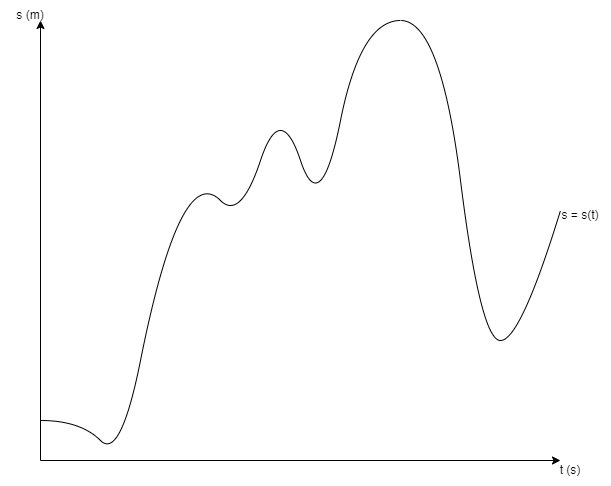
\includegraphics[scale=0.6]{s-t graph.png}
    \end{figure}

    若欲求得任意時間的位移,考慮在極短時間内的瞬間位移相等於瞬時速度乘以時間跨度:設$s(t):(0,\infty)\to\mathbb{R}$為位移函數,則$$\Delta s(t)=v(t)\Delta t$$ 并且總位移應由所有所有瞬間的瞬間位移總和得出,則可考慮將時間均分爲$n$段瞬間,記$t=0$為初始時間及$t_f$為終結時間,并且$0=t_0<t_1<t_2<\cdots<t_n=t_f$,並記對其求和:$$s(t_f)=\sum_{k=0}^{n-1}(s(t_{k+1})-s(t_k))=\sum_{k=0}^{n-1}v(t_k)(t_{k+1}-t_k)$$
    
    \begin{figure}[H]
        \centering
        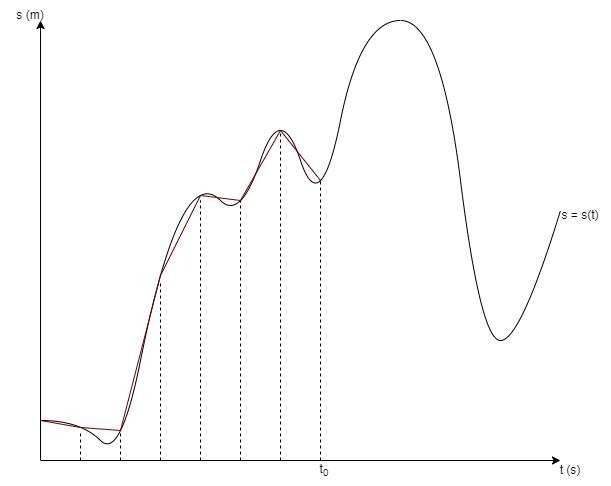
\includegraphics[scale=0.6]{partition s-t.png}
    \end{figure}

    將$n\to\infty$便可定義$$s(t_f)=\int_{0}^{t_f}v(t)dt$$若視$t_f$為變量,則稱其爲\textbf{不定積分};反之,則稱其爲\textbf{定積分}。
    
    \section*{積分的含義}
    從以上簡介可以看出,積分的目的在於加法;更明確的説法是定積分在於計算面積。與中學教程不同,我們會先觀察定積分,再闡述不定積分(實際上他們只差一步)。

    \subsection*{黎曼積分法}
    黎曼對於曲綫下的面積有著相當扎實的幾何見解,他認爲每一條連續曲綫都可以用分割法的方式進行求積,而且\textbf{無論分割的方法如何隨機,若分割數量趨向無限,其結果都是恆定的}。

    藉著以上見解,黎曼將某區間$[a,b]$拆分爲$n$個區間,使得$a=a_0<a_1<a_2<\cdots<a_n=b$並記第$k$個區間為$$P_k:=[a_{k-1},a_k]$$因應$P_k$的有限性及函數$f$的連續性,隨機於$P_k$内抽取變量$t_k\in P_k=[a_{k-1},a_k]$,可得對於$P_k$上的曲綫面積的估算$$f(t_k)\norm*{P_k}$$其中$\norm*{P_k}$代表區間$P_k$的寬度。更進一步可定義$$\norm*{P}:=\max{\norm*{P_k}}$$因此,黎曼給出的積分方法如下

    \begin{definition}[黎曼積分]
        設$f$為$[a,b]$上的連續函數,令存在$a_1,a_2,\dots,a_{n-1}$使得$a=:a_0<a_1<a_2<\cdots<a_n:=b$,並設$P:=\{(t_k,P_k):1\leq k\leq n\}$為\textbf{標識區間集}使得$t_k\in P_k=[a_{k-1},a_k]$,則定義$f$在$[a,b]$上的\textbf{$P$-估算面積}為$$S(f;P):=\sum_{k=1}^{n}f(t_k)\norm*{P}$$
        而精確面積為$$\int_{a}^{b}f=S(f):=\lim_{n\to \infty}S(f;P)$$
    \end{definition}

    另外,若存在$L\in \mathbb{R}$使得對於$\varepsilon>0$,$|\int_a^b f - L| < \varepsilon$,則稱$f$為\textbf{黎曼可積}的函數,記爲$f\in\mathcal{R}[a,b]$。

    黎曼積分屬於概念上的積分,實際情況還需要確定一種$t_k$的取值方法。我們先論證黎曼積分的存在性和唯一性,再討論實際應用會如何處理。

    \begin{theorem}
        若$f$為有限區間内的連續函數,則$f$的黎曼積分有界且唯一。
    \end{theorem}
    \begin{proof}
        由於\begin{align*}
            \min\{\sum_{k=1}^{n}f(t_k)\norm*{P}\}\leq \sum_{k=1}^{n}f(t_k)\norm*{P}\leq \max\{\sum_{k=1}^{n}f(t_k)\norm*{P}\}\\
            \sum_{k=1}^{n}\min\{f(t_k)\}\norm*{P}\leq \sum_{k=1}^{n}f(t_k)\norm*{P}\leq \sum_{k=1}^{n}\max\{f(t_k)\}\norm*{P}
        \end{align*}
        因此\begin{align*}
            \lim_{n\to\infty}\sum_{k=1}^{n}\min\{f(t_k)\}\norm*{P}\leq \lim_{n\to\infty}\sum_{k=1}^{n}f(t_k)\norm*{P}\leq \lim_{n\to\infty}\sum_{k=1}^{n}\max\{f(t_k)\}\norm*{P}
        \end{align*}
        對於$\norm*{P}\to 0$,可視$\min\{f(t_k)\}=\max\{f(t_k)\}$,因此$\int_{a}^{b}f$唯一存在。
    \end{proof}

    由於黎曼積分的定義基於幾何分割而定,因此初始的黎曼積分存在許多不確定性。后經過一系列修訂,終於發展一些可用理論。

    \begin{theorem}
        若$g\in\mathcal{R}[a,b]$且除了有限點以外$f=g$成立,則$f\in\mathcal{R}[a,b]$而且$\int_a^b f = \int_a^b g$。
    \end{theorem}

    \begin{proof}
        證明可拆分爲兩部分,先證明對於一個不等點理論成立,隨後以歸納法論證。

        設$c\in(a,b)$並設$L=\int_a^b g$。設當$x\neq c$時$f(x)=g(x)$。對於任意標識區間集,$S(f;P)=S(f;P)$除了至多兩項,即$$[\cdot,c], [c,\cdot]$$因此\begin{align*}
            |S(f;P)-S(g;P)|&=|\sum (f(x_i)-g(x_i))(x_i-x_{i-1})|\\
            &=|(f(c)-g(c))(c-x_{k-1})+(f(c)-g(c))(x_{k+1}-c)|\\
            &<2(|f(c)|+|g(c)|)\norm*{P}
        \end{align*}

        由此設$\varepsilon>0$,$\delta_1<\frac{\varepsilon}{4(f(|c|)+|g(c)|)}$,以及$\norm*{P}<\delta_2$使得$|S(g;P)-L|<\frac{\varepsilon}{2}$。由此設$\delta<\min\{\delta_1,\delta_2\}$可得\begin{align*}
            |S(f;P)-L|&<|S(f;P)-S(g;P)|+|S(g;P)-L|\\
            &<\frac{\varepsilon}{2}+\frac{\varepsilon}{2}\\
            &=\varepsilon
        \end{align*}
        因此,$f\in\mathcal{R}[a,b]$。

        利用歸納法,不難得出對於有$n$個不等點的情況,把$[a,b]$拆分爲$[a,c]$及$[c,b]$使得$[a,c]$上有$n-1$個不等點,由此證畢。
    \end{proof}

    既然黎曼積分肯定有唯一值,那麽如何計算就成爲了一大問題,畢竟黎曼所提出的概念本就相當抽象,隨機取值雖然可以概括算法,但人類不能將之有效計算。我們給出下列普遍算法,以確定黎曼積分的值。

    以下考慮函數$y=x^2$在$[-1,1]$區間的值。

    \subsubsection*{左取值法}

    對於每一個分區間$[x_i,x_{i+1}]$,取$f(x_i)$作計算值,則寫$$\int_a^b f=\sum f(x_i)\norm*{P}$$

    \begin{example}
        設$f(x)=x^2$,則\begin{align*}
            S(f;P)&=\sum_{i=0}^{2n-1} (x_i^2) \frac{1}{n}\\
            &=\frac{1}{n}[(-1)^2+(\frac{1-n}{n})^2+\cdots+(\frac{n-1}{n})^2]\\
            &=\frac{1}{n}[0^2+2\cdot (\frac{1}{n})^2+\cdots+2\cdot 1^2 - 1^2]\\
            &=\frac{1}{n^3}[2(1^2+2^2+\cdots +n^2)-n^2]\\
            &=\frac{1}{n^3}[2\cdot \frac{1}{6}(n)(n+1)(2n+1)-n^2]\\
            &=\frac{2}{3}+\mathcal{O}(\frac{1}{n})
        \end{align*}
        因此,$\displaystyle\int_{-1}^1 f = \lim_{n\to \infty}S(f;P)=\frac{2}{3}$.
    \end{example}

    \subsubsection*{右取值法}

    對於每一個分區間$[x_i,x_{i+1}]$,取$f(x_{i+1})$作計算值,則寫$$\int_a^b f=\sum f(x_{i+1})\norm*{P}$$

    \begin{example}
        設$f(x)=x^2$,則\begin{align*}
            S(f;P)&=\sum_{i=0}^{2n-1} (x_{i+1}^2) \frac{1}{n}\\
            &=\frac{1}{n}[(\frac{1-n}{n})^2+\cdots+(\frac{n-1}{n})^2+1^2]\\
            &=\frac{1}{n}[0^2+2\cdot (\frac{1}{n})^2+\cdots+2\cdot 1^2 - 1^2]\\
            &=\frac{1}{n^3}[2(1^2+2^2+\cdots +n^2)-n^2]\\
            &=\frac{1}{n^3}[2\cdot \frac{1}{6}(n)(n+1)(2n+1)-n^2]\\
            &=\frac{2}{3}+\mathcal{O}(\frac{1}{n})
        \end{align*}
        因此,$\displaystyle\int_{-1}^1 f = \lim_{n\to \infty}S(f;P)=\frac{2}{3}$.
    \end{example}
    \subsubsection*{中取值法}

    對於每一個分區間$[x_i,x_{i+1}]$,取$f(\frac{x_i+x_{i+1}}{2})$作計算值,則寫$$\int_a^b f=\sum f(\frac{x_i+x_{i+1}}{2})\norm*{P}$$

    \begin{example}
        設$f(x)=x^2$,則\begin{align*}
            S(f;P)&=\sum_{i=0}^{2n-1} (\frac{x_i+x_{i+1}}{2})^2 \frac{1}{n}\\
            &=\frac{1}{n}[(\frac{1-2n}{2n})^2+(\frac{3-2n}{2n})^2+\cdots+(\frac{2n-1}{2n})^2]\\
            &=\frac{1}{n}[2\cdot (\frac{1}{2n})^2+\cdots+2\cdot (\frac{2n-1}{2n})^2]\\
            &=\frac{1}{2n^3}[(1^2+3^2+\cdots +(2n-1)^2)]\\
            &=\frac{1}{2n^3}[\frac{1}{6}(2n)(2n+1)(4n+1)-4\cdot\frac{1}{6}(n)(n+1)(2n+1)]\\
            &=\frac{1}{12n^3}(2n+1)[(2n)(4n+1)-4(n)(n+1)]\\
            &=\frac{1}{6n^3}(2n+1)(2n-1)(n)\\
            &=\frac{2}{3}+\mathcal{O}(\frac{1}{n})
        \end{align*}
        因此,$\displaystyle\int_{-1}^1 f = \lim_{n\to \infty}S(f;P)=\frac{2}{3}$.
    \end{example}
    \subsubsection*{梯形法則}
    對於每一個分區間$[x_i,x_{i+1}]$,取$\frac{f(x_i)+f(x_{i+1})}{2}$作計算值,則寫$$\int_a^b f=\sum \frac{f(x_i)+f(x_{i+1})}{2}\norm*{P}$$

    \begin{example}
        設$f(x)=x^2$,則\begin{align*}
            S(f;P)&=\sum_{i=0}^{2n-1} \frac{x_i^2+x_{i+1}^2}{2} \frac{1}{n}\\
            &=\frac{1}{2}(\textrm{左和}+\textrm{右和})\\
            &=\frac{1}{2}(\frac{2}{3}+\frac{2}{3}+\mathcal{O}(\frac{1}{n}))\\
            &=\frac{2}{3}+\mathcal{O}(\frac{1}{n})
        \end{align*}
        因此,$\displaystyle\int_{-1}^1 f = \lim_{n\to \infty}S(f;P)=\frac{2}{3}$.
    \end{example}
    \subsection*{勒貝格積分法}
    \subsection*{萊布尼茨法則}
    \section*{積分方法}
    \subsection*{基本積分定則}
    \subsection*{換元代入法}
    \subsection*{參數化代入法}
    \subsection*{部分積分法}
    \subsection*{費曼積分法}
    \section*{體積運算}
    \subsection*{圓盤法}
    \subsection*{外殼法}
    \section*{多元積分}
    \subsection*{雙重積分}
    \subsection*{三重積分}
    \section*{向量函數積分}
    \subsection*{綫積分}
    \subsection*{曲面積分}
\end{document}